\documentclass[12pt,a4paper]{article}

\usepackage{setspace}
\onehalfspacing
\usepackage{caption}
\usepackage{subcaption}
\usepackage{float}
\captionsetup[table]{font={stretch=1.5}}     %% change 1.5 as you like
\captionsetup[figure]{font=onehalfspacing}    %% change onehalfspacing as you like
\usepackage[english]{babel}
\usepackage[utf8]{inputenc}
\usepackage{amsmath}
\usepackage{mathtools}
\usepackage{amssymb}
\usepackage{graphicx}
\usepackage{braket}
\usepackage[colorinlistoftodos]{todonotes}
\usepackage[top=1.0in,left=1.0in,right=1.0in,bottom=1.0in]{geometry}
\usepackage[
backend=biber,
style=numeric,
citestyle=ieee,
subentry,
mcite=true,
]{biblatex} %biblatex, more modern form of bibtex 
\usepackage{multicol,caption}
\usepackage{makeidx}
\usepackage{pdfpages}
\usepackage[compat=1.0.0]{tikz-feynman}
\usepackage{hyperref}
%\usepackage{LuaLaTeX}
\makeindex
%\usepackage{fixltx2e}
%\usepackage{cite} %if you want to use bibtex
\newenvironment{Figure}
  {\par\medskip\noindent\minipage{\linewidth}}
  {\endminipage\par\medskip}
\setlength{\columnsep}{1cm}
\setlength{\parindent}{0pt}
\usepackage{color,soul}
\usepackage{booktabs}
\newcommand{\ra}[1]{\renewcommand{\arraystretch}{#1}}
\defbibentryset{griffiths2008book}{griffiths2008introduction, griffiths2008neutrino1.5, griffiths2008neutrinoOscillations} %if you want to use biblatex with multiple referances, useful for books
\addbibresource{refs.bib} %if you want to use bib latex, add sources
\setlength\bibitemsep{2.0\itemsep} % if you want to use bib latex and increase item seperation

\title{Rough Thesis}
\date{\today}
\author{Ronald Collins ID:200948843}

\begin{document}
\maketitle

\begin{Figure}
 \centering
 
\includegraphics[width=1.0\linewidth]{Liverpool_logo}
 \captionof*{figure}{} 
\end{Figure}


\begin{center}
\textit{Department of Physics, High Energy Physics\\}
\textit{VIDARR collaboration\\}
\end{center}


\pagenumbering{gobble}
\newpage
\pagenumbering{roman}
\begin{abstract}
\normalsize A basic overview\\

\providecommand{\keywords}[1]{\textbf{\textit{Keywords:}} #1} %Keywords command has to be supplied manually
\keywords{Monte Carlo, Geant4, High performance computing (HPC), Anti-neutrino}
\end{abstract}
\vspace{5mm} %5mm vertical space before main body of text
%\begin{multicols}{2}
\tableofcontents
\newpage

\pagenumbering{arabic}

\section{The Aim Of VIDARR} \label{sec_theAimOfVidarr}
The aim of the VIDARR project is to demonstrate the potential usefulness of a plastic scintillating detector for safeguarding purposes. To that end the characterisation and simulation of two versions of the detector will be used in order to show the full potential of this idea. Reactor monitoring using $\Bar{\nu_e}$ was suggested as early as 1978 \cite{Borovoi_1978} but the political climate of the cold war era prevent interest in the technology from being fully realised. In the modern political climate where nuclear power is seen as a stable form of low carbon power generation more nations are considering the technology once again. And as such the concern of the proliferation of atomic weapons has increased. Current methods of non-proliferation are dependent on accurate bookkeeping and empirical measurement estimations from power generation. Whilst these methods are effective more direct methods of measuring the flux from reactors and thereby the production of weapons grade material would greatly aid in the trust between nations and help to prevent the spread of atomic weaponry. 
\\\\This technology also has benefits for increasing the burn-up of nuclear waste which could increase power generation at nuclear power plants and reduce the production of nuclear waste which has to be stored. This potential is not yet fully realised due to the increased complexity of the method as it requires differentiating between different isotopes rather than just measuring flux. Tough this should be feasible it is not possible to test this capability until the upgraded VIDARR detector is deployed at a reactor site. 

\section{The Prototype Detector}\label{sec_thePrototypeDetector}
This thesis will cover two distinct versions of the detector. The original prototype detector which was re-purposed technology from the T2K ND280 ECal \cite{Allan_2013} and an upgraded version which uses the same basic materials in the detector but upgraded electronics and containment which will be refereed to as the ``Verification Instrument for Direct Assay of Nuclear Reactors at Range'' (VIDARR) detector. The rest of this section will focus on the prototype detector.
\\\\As it is the basis for the other detectors a quick overview of the T2K ND280 ECal will be required. The ND280 is series of detectors from the neutrino oscillation experiment T2K which relies on a $\mu_nu$ beam entering the detector as show in figure \ref{fig_nd280Fig}. This detector was comprised of several different types of detector including time projection chambers (TPCs) and fine-grained detectors (FGDs) and electromagnetic calorimeters (ECals) \cite{Allan_2013}. The ECals are of particular interest as they are the basis for the prototype and VIDARR detectors. 
\begin{figure}[H]
 \centering
 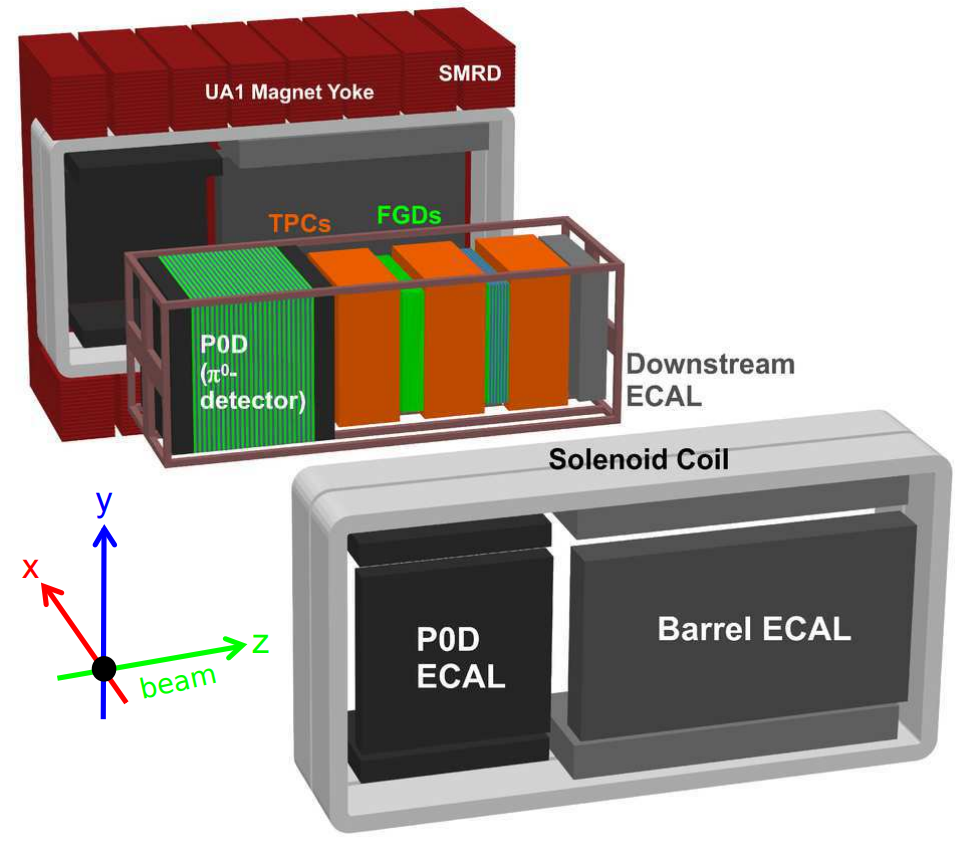
\includegraphics[width=\linewidth/2]{ND280Fig.png} 
 \captionof{figure}{Diagram of the ND280 detector. From \cite{Allan_2013}} %~can be used as a kind of place holder in latex
 \label{fig_nd280Fig}
\end{figure}
The T2K Ecals were made from plastic scintillating bars measuring 4\,cm by 1\,cm with varying lengths arranged in alternating layers at 90 degrees to each other \cite{Allan_2013}. Wavelength shifting (wls) fibres were placed in the centre of the scintillating bars which shift the wavelength from blue to green \cite{Allan_2013}. These wavelength shifting fibres are then connected to multi-pixel photon counters (MPPCs) which are the instrument which reads out the signal. This signal is then read in by Trip-T front-end electronic boards (TFBs) which then splits the signal into different cycles each containing 1.5 microseconds of information. All of this is shared by the prototype detector. 
\\\\However a crucial different between the ECals of the ND280 and the prototype detector is that the (ECals) had a layer of lead in between each of the plastic scintillating layers \cite{Allan_2013}. In the prototype this has been replaced with a layer of gadolinium so that neutrons were capture for inverse $\beta$ decay. The prototype was also designed to fit inside of a shipping container each bar having a length of 152\,cm and the whole detector measuring 152\,cm by 152\,cm with 49 layers of plastic scintillating bars totalling 49\,cm. The electronic systems were also adapted from the from the T2K system however they were altered such that they triggered on a gadolinium cascade from inverse $\beta$ decay. There were 23 cycles numbered from 0-22 with 0-17 cycles being considered "prompt" and cycle 18 is the trigger cycle. Cycles 19 -22 were left alone so that they could be compared in case time dependent issues arose from the altered system. Cycles 19-22 are useful for $\mu$ tomography as time dependent errors can arise from this adaptation of the electronics. 
\\\\The original detector was deployed at Wylfa power station in Anglesey Wales for an 18-month period. This run proved successful measuring the power on from the reactor to within good agreement to the measured reactor flux see figure \ref{fig_prototypeMeasumentFlux}. With a measured anti-neutrino rate of 172.1 $\pm$ 4.6 candidates per day when the reactor is off and 203.7 $\pm$ 19.6 when the reactor was on \cite{Carroll_2018}. Unfortunately due to cooling issues with the prototype the reactor shutdown was not observed. This is one of the main motivating factors behind the upgrade of the detector as the first generation MPPCs and reporposed electronics were susceptible to high levels of noise if the temperature was not carefully controlled. 
\begin{figure}[H]
 \centering
 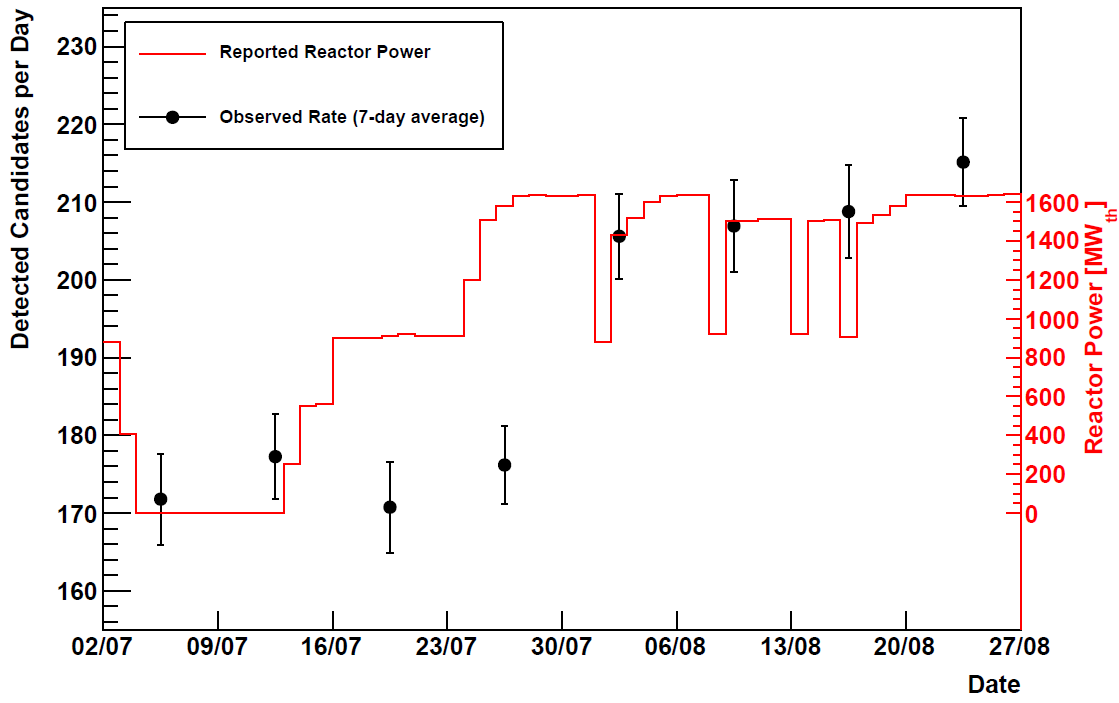
\includegraphics[width=0.90\linewidth]{prototypeMeasureOnFig.png} 
 \captionof{figure}{Measured anti-neutrino flux compared to the power generation from the Wylfa power station. From \cite{Carroll_2018}} %~can be used as a kind of place holder in latex
 \label{fig_prototypeMeasumentFlux}
\end{figure}
\section{The Upgraded Detector}\label{sec_theUpgradedDetector}
Please note that in the following section of text the term upgraded and VIDARR detector are used interchangeably. The upgraded detector will have 21 more layers than the previous detector going from 49 to 70 layers and the 3 missing columns in side a are also now instrumented. This means the number of channels have increased from 1793 to 2660 which results in an increase of mass by $\sim$ 50\,\%, thus improving the fiducial volume of the detector. This means that more energy from the gadolinium cascade is contained within the detector thus allowing for more effective noise reduction when triggering. Therefore the increase in layers will allow for a higher efficiency of neutron capture. The increase in layers will not yield a significant increase in positron efficiency as positrons are effectively contained to a $\sim$ 99\,\% level with both 1793 channels and 2660 channels as they are contained within 1-2 bars.
\\\\The electronics have also been improved significantly compared to the original detector. The original electronics were carried over from the T2K Ecal, they were the first generation of the technology with relatively high noise rates compared to the current generation used in the VIDARR detector. The energy resolution of the electronics have been greatly increased \hl{(any quantifiable numbers for this stuff?)}. And the noise rates for the original electronics were also more susceptible to changes in temperature than the electronics in the upgraded detector. In addition the upgraded detector will also have field-programmable gate array (FPGA) boards which connect with analogue boards which in turn connect to the MPPCs. The use of FPGA boards allow for more complex trigger functions to be used with up to two thresholds to be used and allows for the summed energy and the number of bars to be hit to be used for trigger discrimination. Which should allow for better signal to noise discrimination than the original detector.
\\\\A basic cut investigation used a form of machine learning called a support vector machine (SVM) to determine the best cut and which dimensions gave the best separation. The cut was dominated by the number of bars hit at the lower threshold of 0.1\,MeV, the most accurate cut would have been utilising the number of bars hit above 0.1\,MeV and the summed energy above the 0.1\,MeV threshold. However due to the structure of the FPGA boards and their programming it was more prudent to use the number of bars hit above both the 0.1\,MeV thresholds and 0.5\,MeV threshold. The cost in classifier accuracy was minimal and it allowed for faster development of the FPGA firmware. 
\\\\To lessen temperature fluctuations in the VIDARR detector the cooling in and around the detector module has been greatly increased from the prototype. The original detector had six radiator fins on 2 sides of the detector which were primarily aimed at cooling the TFBs on each fin. The upgraded VIDARR detector will also have these fins which will help cool the new boards but on the same 2 sides as the fins there will also be two new radiators behind the fins which run the width and height of a side. Greatly increasing the speed that heat will dissipate inside the detector. This will allow for a more consistent temperature  thus reducing dark noise even further from the MPPCs. 
\section{Geant 4 Simulation}\label{sec_geant4Simulation} 
The VIDARR detector is also represented in a GEANT4 simulation which is a provident physics simulation package. According to the GEANT4 collaboration GEANT4 ``covers a comprehensive range including electromagnetic, hadronic and optical processes and a large set of long-lived particles materials and elements over a wide energy range starting in some cases from 250\,eV and extending in others to the TeV range'' \cite{Agostinelli:2002hh}. Considering that the energy range for inverse $\beta$ decay is 2\,MeV-8\,MeV \cite{Mueller_2011} this simulation package appears to meet the needs of the VIDARR collaboration. However whilst the simulation of the resulting positrons is reasonably simplistic the simulation of the neutrons is more challenging due to the difficulty in simulating the Gadolinium cascade. 
\\\\The Gadolinium cascade is difficult to measure and accurately simulate for for two main reasons. The first is that the gadolinium nuclei that have good neutron capture are isotopes $^{155}$Gd and $^{157}$Gd which have 155 and 157 nucleons respectively. Both of these nuclei are large and as such it is difficult to accurately model the individual interactions between each of the nucleons. So, there is no agreed upon model at present for the absorption and emission of the 8\,MeV $\gamma$ cascade. The second issue is that the high energy $\gamma$ rays emitted by the cascade are very difficult to contain. Therefore, getting accurate measurements and energy efficiencies for the cascade is also very difficult. These two problems compound one another it is difficult to measure the cascade so it is difficult to model which, in turn, makes it difficult to know the energies expected to be emitted by the nuclei. Further issues are caused by highly penetrative making efficiency estimates even less accurate. \hl{(No references... whilst this is all reasonably straight forward some more concrete numbers and figures would be nice...)}. Gadolinium is used because of its high efficiency (10$\%$ - 40$\%$) compared to other neutron capturing materials such as $^6$Li which only has about $1\%$ \cite{Abdushukurov_2010}. 
\\\\The simulation has several distinct modes: cosmic $\mu$, noise, and inverse $\beta$ decay. The cosmic mode has a realistic distribution \hl{what paper did Matt Murdock use to form the realistic distribution?} and a cosmic hemisphere distribution. The cosmic hemisphere distribution is used to check that the analysis chain is functioning as expected and for testing simulated reactor shadows. In all other cases the realistic cosmic distribution is used when simulating cosmic $mu$s. The noise distributions are random uniform distributions from 0 - 10\,MeV simulating which cover $p$,$\bar{p}$,$\pi^+$,$\pi^-$,$e^-$,$e^+$, $\alpha$,$\bar{\alpha}$,$n$. The IBD simulation is done by simulating a positron between 0 - 10\,MeV and then simulating at $\sim$ 10 $\mu$s later a neutron. \hl{Timing plot required!}. The range 0 - 10\,MeV is used instead of 2 - 8\,MeV to allow the testing of edge cases and for better fitting and or particle identification later down the road. \hl{need figures for both cosmic and ibd, this requires access to OLL however...}.
\\\\In order to characterise the physical effects of the detector at test stand was set up by fellow collaborator George Holt. This test stand contained a single plastic scintillating bar where a caesium 137 source was placed at 11 intervals across the bar from which attenuation of the 662\,KeV peak could then be measured. This is then shown in figure \ref{fig_attenuationPlot} this exponential decay is then put into the simulation so that the amount of light produced is more physical. The other characterisation was done via 
\begin{figure}[H]
 \centering
 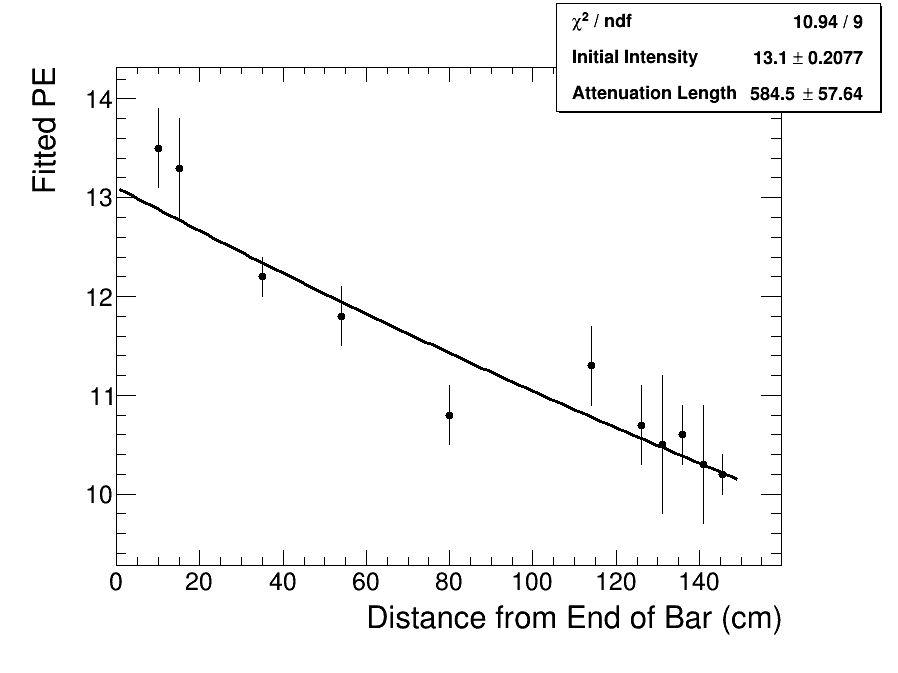
\includegraphics[width=1.0\linewidth]{result_from_attnPlotter.png} 
 \captionof{figure}{The attenuation plot for test stand produced by George Holt. The attenution length is 580 $\pm$ 60 \hl{units!}} %~can be used as a kind of place holder in latex
 \label{fig_attenuationPlot}
\end{figure}
\section{Cosmic Tomography}\label{sec_cosmicTomography}
\subsection{Simulation}\label{subSec_cosmicTomography_simulation}
\subsection{Methodology}\label{subSec_cosmicTomography_methodology}

%\bibliography{refs} 
%\bibliographystyle{ieeetr}
\printbibliography


\end{document}
